% Created by tikzDevice version 0.12.3 on 2020-12-23 20:24:03
% !TEX encoding = UTF-8 Unicode
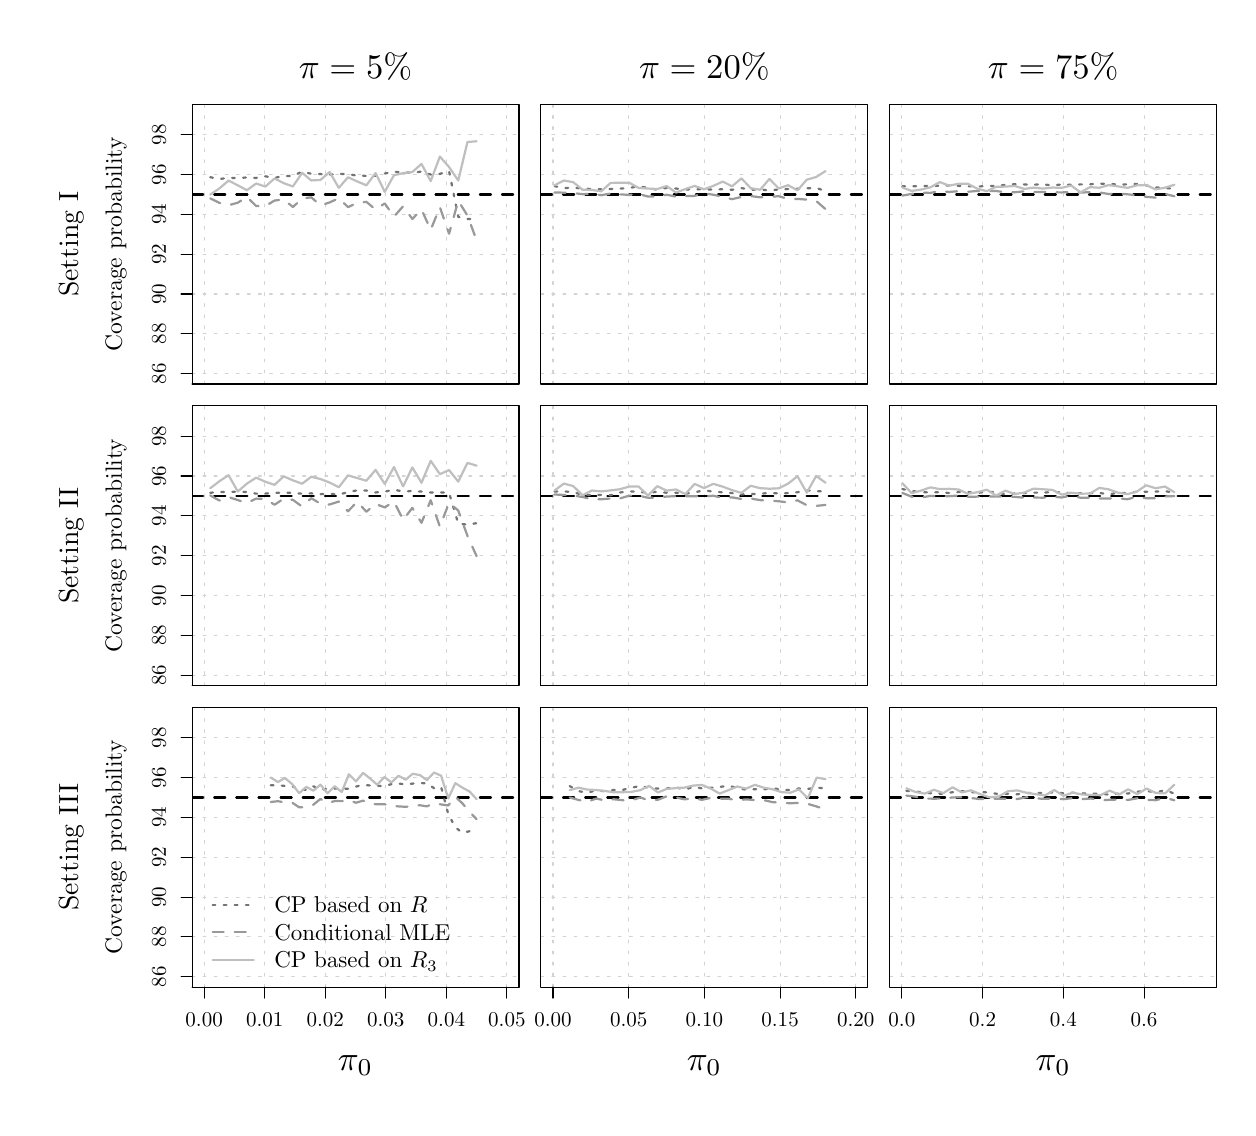
\begin{tikzpicture}[x=1pt,y=1pt]
\definecolor{fillColor}{RGB}{255,255,255}
\path[use as bounding box,fill=fillColor,fill opacity=0.00] (0,0) rectangle (433.62,390.26);
\begin{scope}
\path[clip] ( 55.44,257.53) rectangle (181.50,366.50);
\definecolor{drawColor}{RGB}{0,0,0}

\node[text=drawColor,anchor=base,inner sep=0pt, outer sep=0pt, scale=  0.66] at (118.47,231.40) {Simulation ID};

\node[text=drawColor,rotate= 90.00,anchor=base,inner sep=0pt, outer sep=0pt, scale=  0.66] at ( 34.06,312.01) {Ratio of RMSE};
\end{scope}
\begin{scope}
\path[clip] (  0.00,  0.00) rectangle (433.62,390.26);
\definecolor{drawColor}{RGB}{0,0,0}

\path[draw=drawColor,line width= 0.4pt,line join=round,line cap=round] ( 59.40,265.23) -- ( 59.40,351.60);

\path[draw=drawColor,line width= 0.4pt,line join=round,line cap=round] ( 59.40,265.23) -- ( 55.44,265.23);

\path[draw=drawColor,line width= 0.4pt,line join=round,line cap=round] ( 59.40,279.63) -- ( 55.44,279.63);

\path[draw=drawColor,line width= 0.4pt,line join=round,line cap=round] ( 59.40,294.02) -- ( 55.44,294.02);

\path[draw=drawColor,line width= 0.4pt,line join=round,line cap=round] ( 59.40,308.42) -- ( 55.44,308.42);

\path[draw=drawColor,line width= 0.4pt,line join=round,line cap=round] ( 59.40,322.81) -- ( 55.44,322.81);

\path[draw=drawColor,line width= 0.4pt,line join=round,line cap=round] ( 59.40,337.20) -- ( 55.44,337.20);

\path[draw=drawColor,line width= 0.4pt,line join=round,line cap=round] ( 59.40,351.60) -- ( 55.44,351.60);

\node[text=drawColor,rotate= 90.00,anchor=base,inner sep=0pt, outer sep=0pt, scale=  0.76] at ( 49.90,265.23) {86};

\node[text=drawColor,rotate= 90.00,anchor=base,inner sep=0pt, outer sep=0pt, scale=  0.76] at ( 49.90,279.63) {88};

\node[text=drawColor,rotate= 90.00,anchor=base,inner sep=0pt, outer sep=0pt, scale=  0.76] at ( 49.90,294.02) {90};

\node[text=drawColor,rotate= 90.00,anchor=base,inner sep=0pt, outer sep=0pt, scale=  0.76] at ( 49.90,308.42) {92};

\node[text=drawColor,rotate= 90.00,anchor=base,inner sep=0pt, outer sep=0pt, scale=  0.76] at ( 49.90,322.81) {94};

\node[text=drawColor,rotate= 90.00,anchor=base,inner sep=0pt, outer sep=0pt, scale=  0.76] at ( 49.90,337.20) {96};

\node[text=drawColor,rotate= 90.00,anchor=base,inner sep=0pt, outer sep=0pt, scale=  0.76] at ( 49.90,351.60) {98};
\end{scope}
\begin{scope}
\path[clip] ( 59.40,261.49) rectangle (177.54,362.54);
\definecolor{drawColor}{RGB}{211,211,211}

\path[draw=drawColor,line width= 0.4pt,dash pattern=on 1pt off 3pt ,line join=round,line cap=round] ( 63.78,261.49) -- ( 63.78,362.54);

\path[draw=drawColor,line width= 0.4pt,dash pattern=on 1pt off 3pt ,line join=round,line cap=round] ( 85.65,261.49) -- ( 85.65,362.54);

\path[draw=drawColor,line width= 0.4pt,dash pattern=on 1pt off 3pt ,line join=round,line cap=round] (107.53,261.49) -- (107.53,362.54);

\path[draw=drawColor,line width= 0.4pt,dash pattern=on 1pt off 3pt ,line join=round,line cap=round] (129.41,261.49) -- (129.41,362.54);

\path[draw=drawColor,line width= 0.4pt,dash pattern=on 1pt off 3pt ,line join=round,line cap=round] (151.29,261.49) -- (151.29,362.54);

\path[draw=drawColor,line width= 0.4pt,dash pattern=on 1pt off 3pt ,line join=round,line cap=round] (173.16,261.49) -- (173.16,362.54);

\path[draw=drawColor,line width= 0.4pt,dash pattern=on 1pt off 3pt ,line join=round,line cap=round] ( 59.40,265.23) -- (177.54,265.23);

\path[draw=drawColor,line width= 0.4pt,dash pattern=on 1pt off 3pt ,line join=round,line cap=round] ( 59.40,279.63) -- (177.54,279.63);

\path[draw=drawColor,line width= 0.4pt,dash pattern=on 1pt off 3pt ,line join=round,line cap=round] ( 59.40,294.02) -- (177.54,294.02);

\path[draw=drawColor,line width= 0.4pt,dash pattern=on 1pt off 3pt ,line join=round,line cap=round] ( 59.40,308.42) -- (177.54,308.42);

\path[draw=drawColor,line width= 0.4pt,dash pattern=on 1pt off 3pt ,line join=round,line cap=round] ( 59.40,322.81) -- (177.54,322.81);

\path[draw=drawColor,line width= 0.4pt,dash pattern=on 1pt off 3pt ,line join=round,line cap=round] ( 59.40,337.20) -- (177.54,337.20);

\path[draw=drawColor,line width= 0.4pt,dash pattern=on 1pt off 3pt ,line join=round,line cap=round] ( 59.40,351.60) -- (177.54,351.60);
\end{scope}
\begin{scope}
\path[clip] (  0.00,  0.00) rectangle (433.62,390.26);
\definecolor{drawColor}{RGB}{0,0,0}

\path[draw=drawColor,line width= 0.4pt,line join=round,line cap=round] ( 59.40,261.49) --
	(177.54,261.49) --
	(177.54,362.54) --
	( 59.40,362.54) --
	( 59.40,261.49);
\end{scope}
\begin{scope}
\path[clip] ( 59.40,261.49) rectangle (177.54,362.54);
\definecolor{drawColor}{RGB}{0,0,0}

\path[draw=drawColor,line width= 0.8pt,dash pattern=on 4pt off 4pt ,line join=round,line cap=round] ( 59.40,330.01) -- (177.54,330.01);
\definecolor{drawColor}{gray}{0.45}

\path[draw=drawColor,line width= 0.8pt,dash pattern=on 1pt off 3pt ,line join=round,line cap=round] ( 65.96,336.23) --
	( 69.28,335.55) --
	( 72.60,336.02) --
	( 75.92,335.89) --
	( 79.24,336.14) --
	( 82.56,335.95) --
	( 85.88,336.54) --
	( 89.20,336.01) --
	( 92.52,336.61) --
	( 95.84,336.64) --
	( 99.16,338.24) --
	(102.48,337.46) --
	(105.80,337.35) --
	(109.12,337.12) --
	(112.43,337.46) --
	(115.75,337.31) --
	(119.07,336.80) --
	(122.39,336.69) --
	(125.71,336.70) --
	(129.03,337.55) --
	(132.35,338.17) --
	(135.67,338.05) --
	(138.99,337.79) --
	(142.31,338.28) --
	(145.63,337.18) --
	(148.95,337.43) --
	(152.27,338.46) --
	(155.59,321.89) --
	(158.91,321.14) --
	(162.23,321.07);
\definecolor{drawColor}{gray}{0.60}

\path[draw=drawColor,line width= 0.8pt,dash pattern=on 4pt off 4pt ,line join=round,line cap=round] ( 65.96,328.58) --
	( 69.28,326.94) --
	( 72.60,326.09) --
	( 75.92,327.01) --
	( 79.24,329.06) --
	( 82.56,325.82) --
	( 85.88,325.78) --
	( 89.20,327.79) --
	( 92.52,328.19) --
	( 95.84,325.46) --
	( 99.16,328.52) --
	(102.48,328.96) --
	(105.80,326.03) --
	(109.12,327.10) --
	(112.43,328.65) --
	(115.75,325.42) --
	(119.07,326.90) --
	(122.39,327.32) --
	(125.71,324.55) --
	(129.03,326.75) --
	(132.35,321.96) --
	(135.67,325.72) --
	(138.99,321.13) --
	(142.31,324.58) --
	(145.63,317.18) --
	(148.95,325.40) --
	(152.27,315.80) --
	(155.59,327.73) --
	(158.91,322.36) --
	(162.23,313.38);
\definecolor{drawColor}{gray}{0.75}

\path[draw=drawColor,line width= 0.8pt,line join=round,line cap=round] ( 65.96,329.91) --
	( 69.28,332.18) --
	( 72.60,335.00) --
	( 75.92,333.29) --
	( 79.24,331.52) --
	( 82.56,333.95) --
	( 85.88,332.84) --
	( 89.20,335.77) --
	( 92.52,334.08) --
	( 95.84,332.87) --
	( 99.16,337.81) --
	(102.48,335.05) --
	(105.80,335.23) --
	(109.12,338.10) --
	(112.43,332.38) --
	(115.75,336.20) --
	(119.07,334.71) --
	(122.39,333.29) --
	(125.71,337.72) --
	(129.03,330.94) --
	(132.35,336.93) --
	(135.67,337.71) --
	(138.99,338.08) --
	(142.31,341.03) --
	(145.63,334.80) --
	(148.95,343.68) --
	(152.27,339.90) --
	(155.59,335.03) --
	(158.91,348.94) --
	(162.23,349.21);
\end{scope}
\begin{scope}
\path[clip] (  0.00,  0.00) rectangle (433.62,390.26);
\definecolor{drawColor}{RGB}{0,0,0}

\node[text=drawColor,rotate= 90.00,anchor=base,inner sep=0pt, outer sep=0pt, scale=  1.00] at ( 18.22,312.01) {Setting I};

\node[text=drawColor,rotate= 90.00,anchor=base,inner sep=0pt, outer sep=0pt, scale=  0.85] at ( 34.06,312.01) {Coverage probability};

\node[text=drawColor,anchor=base,inner sep=0pt, outer sep=0pt, scale=  1.25] at (118.47,372.04) {$\pi = 5\%$};
\end{scope}
\begin{scope}
\path[clip] (181.50,257.53) rectangle (307.56,366.50);
\definecolor{drawColor}{RGB}{0,0,0}

\node[text=drawColor,anchor=base,inner sep=0pt, outer sep=0pt, scale=  0.66] at (244.53,231.40) {Simulation ID};

\node[text=drawColor,rotate= 90.00,anchor=base,inner sep=0pt, outer sep=0pt, scale=  0.66] at (160.12,312.01) {Ratio of RMSE};
\end{scope}
\begin{scope}
\path[clip] (185.46,261.49) rectangle (303.60,362.54);
\definecolor{drawColor}{RGB}{211,211,211}

\path[draw=drawColor,line width= 0.4pt,dash pattern=on 1pt off 3pt ,line join=round,line cap=round] (189.84,261.49) -- (189.84,362.54);

\path[draw=drawColor,line width= 0.4pt,dash pattern=on 1pt off 3pt ,line join=round,line cap=round] (217.18,261.49) -- (217.18,362.54);

\path[draw=drawColor,line width= 0.4pt,dash pattern=on 1pt off 3pt ,line join=round,line cap=round] (244.53,261.49) -- (244.53,362.54);

\path[draw=drawColor,line width= 0.4pt,dash pattern=on 1pt off 3pt ,line join=round,line cap=round] (271.88,261.49) -- (271.88,362.54);

\path[draw=drawColor,line width= 0.4pt,dash pattern=on 1pt off 3pt ,line join=round,line cap=round] (299.22,261.49) -- (299.22,362.54);

\path[draw=drawColor,line width= 0.4pt,dash pattern=on 1pt off 3pt ,line join=round,line cap=round] (185.46,265.23) -- (303.60,265.23);

\path[draw=drawColor,line width= 0.4pt,dash pattern=on 1pt off 3pt ,line join=round,line cap=round] (185.46,279.63) -- (303.60,279.63);

\path[draw=drawColor,line width= 0.4pt,dash pattern=on 1pt off 3pt ,line join=round,line cap=round] (185.46,294.02) -- (303.60,294.02);

\path[draw=drawColor,line width= 0.4pt,dash pattern=on 1pt off 3pt ,line join=round,line cap=round] (185.46,308.42) -- (303.60,308.42);

\path[draw=drawColor,line width= 0.4pt,dash pattern=on 1pt off 3pt ,line join=round,line cap=round] (185.46,322.81) -- (303.60,322.81);

\path[draw=drawColor,line width= 0.4pt,dash pattern=on 1pt off 3pt ,line join=round,line cap=round] (185.46,337.20) -- (303.60,337.20);

\path[draw=drawColor,line width= 0.4pt,dash pattern=on 1pt off 3pt ,line join=round,line cap=round] (185.46,351.60) -- (303.60,351.60);
\end{scope}
\begin{scope}
\path[clip] (  0.00,  0.00) rectangle (433.62,390.26);
\definecolor{drawColor}{RGB}{0,0,0}

\path[draw=drawColor,line width= 0.4pt,line join=round,line cap=round] (185.46,261.49) --
	(303.60,261.49) --
	(303.60,362.54) --
	(185.46,362.54) --
	(185.46,261.49);
\end{scope}
\begin{scope}
\path[clip] (185.46,261.49) rectangle (303.60,362.54);
\definecolor{drawColor}{RGB}{0,0,0}

\path[draw=drawColor,line width= 0.8pt,dash pattern=on 4pt off 4pt ,line join=round,line cap=round] (185.46,330.01) -- (303.60,330.01);
\definecolor{drawColor}{gray}{0.45}

\path[draw=drawColor,line width= 0.8pt,dash pattern=on 1pt off 3pt ,line join=round,line cap=round] (190.38,333.00) --
	(193.76,332.28) --
	(197.13,332.48) --
	(200.51,332.08) --
	(203.89,331.97) --
	(207.26,331.88) --
	(210.64,331.97) --
	(214.01,332.11) --
	(217.39,332.32) --
	(220.77,332.94) --
	(224.14,332.38) --
	(227.52,331.68) --
	(230.89,332.37) --
	(234.27,332.12) --
	(237.65,331.78) --
	(241.02,331.88) --
	(244.40,331.84) --
	(247.77,331.75) --
	(251.15,331.86) --
	(254.53,331.68) --
	(257.90,332.30) --
	(261.28,331.68) --
	(264.65,331.81) --
	(268.03,331.40) --
	(271.41,331.81) --
	(274.78,331.94) --
	(278.16,332.04) --
	(281.53,332.24) --
	(284.91,332.32) --
	(288.29,331.27);
\definecolor{drawColor}{gray}{0.60}

\path[draw=drawColor,line width= 0.8pt,dash pattern=on 4pt off 4pt ,line join=round,line cap=round] (190.38,330.73) --
	(193.76,330.63) --
	(197.13,330.50) --
	(200.51,330.09) --
	(203.89,330.19) --
	(207.26,329.73) --
	(210.64,330.31) --
	(214.01,330.04) --
	(217.39,329.82) --
	(220.77,330.17) --
	(224.14,329.24) --
	(227.52,329.22) --
	(230.89,329.89) --
	(234.27,329.20) --
	(237.65,329.37) --
	(241.02,329.47) --
	(244.40,330.38) --
	(247.77,329.89) --
	(251.15,329.16) --
	(254.53,328.28) --
	(257.90,329.10) --
	(261.28,329.40) --
	(264.65,328.97) --
	(268.03,329.16) --
	(271.41,329.35) --
	(274.78,328.38) --
	(278.16,328.38) --
	(281.53,328.12) --
	(284.91,327.65) --
	(288.29,324.70);
\definecolor{drawColor}{gray}{0.75}

\path[draw=drawColor,line width= 0.8pt,line join=round,line cap=round] (190.38,333.32) --
	(193.76,335.03) --
	(197.13,334.43) --
	(200.51,331.69) --
	(203.89,331.62) --
	(207.26,331.13) --
	(210.64,334.17) --
	(214.01,334.20) --
	(217.39,334.20) --
	(220.77,332.35) --
	(224.14,332.12) --
	(227.52,331.95) --
	(230.89,333.04) --
	(234.27,330.67) --
	(237.65,331.95) --
	(241.02,333.06) --
	(244.40,331.86) --
	(247.77,333.10) --
	(251.15,334.64) --
	(254.53,332.93) --
	(257.90,335.81) --
	(261.28,332.25) --
	(264.65,331.69) --
	(268.03,335.58) --
	(271.41,332.18) --
	(274.78,333.33) --
	(278.16,331.48) --
	(281.53,335.33) --
	(284.91,336.28) --
	(288.29,338.43);
\end{scope}
\begin{scope}
\path[clip] (  0.00,  0.00) rectangle (433.62,390.26);
\definecolor{drawColor}{RGB}{0,0,0}

\node[text=drawColor,anchor=base,inner sep=0pt, outer sep=0pt, scale=  1.25] at (244.53,372.04) {$\pi= 20\%$};
\end{scope}
\begin{scope}
\path[clip] (307.56,257.53) rectangle (433.62,366.50);
\definecolor{drawColor}{RGB}{0,0,0}

\node[text=drawColor,anchor=base,inner sep=0pt, outer sep=0pt, scale=  0.66] at (370.59,231.40) {Simulation ID};

\node[text=drawColor,rotate= 90.00,anchor=base,inner sep=0pt, outer sep=0pt, scale=  0.66] at (286.18,312.01) {Ratio of RMSE};
\end{scope}
\begin{scope}
\path[clip] (311.52,261.49) rectangle (429.66,362.54);
\definecolor{drawColor}{RGB}{211,211,211}

\path[draw=drawColor,line width= 0.4pt,dash pattern=on 1pt off 3pt ,line join=round,line cap=round] (315.90,261.49) -- (315.90,362.54);

\path[draw=drawColor,line width= 0.4pt,dash pattern=on 1pt off 3pt ,line join=round,line cap=round] (345.07,261.49) -- (345.07,362.54);

\path[draw=drawColor,line width= 0.4pt,dash pattern=on 1pt off 3pt ,line join=round,line cap=round] (374.24,261.49) -- (374.24,362.54);

\path[draw=drawColor,line width= 0.4pt,dash pattern=on 1pt off 3pt ,line join=round,line cap=round] (403.41,261.49) -- (403.41,362.54);

\path[draw=drawColor,line width= 0.4pt,dash pattern=on 1pt off 3pt ,line join=round,line cap=round] (311.52,265.23) -- (429.66,265.23);

\path[draw=drawColor,line width= 0.4pt,dash pattern=on 1pt off 3pt ,line join=round,line cap=round] (311.52,279.63) -- (429.66,279.63);

\path[draw=drawColor,line width= 0.4pt,dash pattern=on 1pt off 3pt ,line join=round,line cap=round] (311.52,294.02) -- (429.66,294.02);

\path[draw=drawColor,line width= 0.4pt,dash pattern=on 1pt off 3pt ,line join=round,line cap=round] (311.52,308.42) -- (429.66,308.42);

\path[draw=drawColor,line width= 0.4pt,dash pattern=on 1pt off 3pt ,line join=round,line cap=round] (311.52,322.81) -- (429.66,322.81);

\path[draw=drawColor,line width= 0.4pt,dash pattern=on 1pt off 3pt ,line join=round,line cap=round] (311.52,337.20) -- (429.66,337.20);

\path[draw=drawColor,line width= 0.4pt,dash pattern=on 1pt off 3pt ,line join=round,line cap=round] (311.52,351.60) -- (429.66,351.60);
\end{scope}
\begin{scope}
\path[clip] (  0.00,  0.00) rectangle (433.62,390.26);
\definecolor{drawColor}{RGB}{0,0,0}

\path[draw=drawColor,line width= 0.4pt,line join=round,line cap=round] (311.52,261.49) --
	(429.66,261.49) --
	(429.66,362.54) --
	(311.52,362.54) --
	(311.52,261.49);
\end{scope}
\begin{scope}
\path[clip] (311.52,261.49) rectangle (429.66,362.54);
\definecolor{drawColor}{RGB}{0,0,0}

\path[draw=drawColor,line width= 0.8pt,dash pattern=on 4pt off 4pt ,line join=round,line cap=round] (311.52,330.01) -- (429.66,330.01);
\definecolor{drawColor}{gray}{0.45}

\path[draw=drawColor,line width= 0.8pt,dash pattern=on 1pt off 3pt ,line join=round,line cap=round] (316.04,332.92) --
	(319.43,332.96) --
	(322.82,332.96) --
	(326.21,333.15) --
	(329.60,333.16) --
	(332.99,333.26) --
	(336.38,333.09) --
	(339.77,332.97) --
	(343.16,332.83) --
	(346.55,333.06) --
	(349.94,333.09) --
	(353.33,333.45) --
	(356.72,333.72) --
	(360.11,333.61) --
	(363.50,333.52) --
	(366.89,333.63) --
	(370.28,333.25) --
	(373.67,333.62) --
	(377.06,333.51) --
	(380.45,333.63) --
	(383.84,333.68) --
	(387.23,333.88) --
	(390.62,333.89) --
	(394.01,333.55) --
	(397.40,333.65) --
	(400.79,333.81) --
	(404.18,333.27) --
	(407.57,332.56) --
	(410.96,332.31) --
	(414.35,332.05);
\definecolor{drawColor}{gray}{0.60}

\path[draw=drawColor,line width= 0.8pt,dash pattern=on 4pt off 4pt ,line join=round,line cap=round] (316.04,329.58) --
	(319.43,330.17) --
	(322.82,330.68) --
	(326.21,330.54) --
	(329.60,331.26) --
	(332.99,330.89) --
	(336.38,331.17) --
	(339.77,330.97) --
	(343.16,331.25) --
	(346.55,331.19) --
	(349.94,331.22) --
	(353.33,330.80) --
	(356.72,330.78) --
	(360.11,331.12) --
	(363.50,330.86) --
	(366.89,330.90) --
	(370.28,330.77) --
	(373.67,330.73) --
	(377.06,330.84) --
	(380.45,330.67) --
	(383.84,330.81) --
	(387.23,330.73) --
	(390.62,330.14) --
	(394.01,330.35) --
	(397.40,330.05) --
	(400.79,329.69) --
	(404.18,329.14) --
	(407.57,328.84) --
	(410.96,330.19) --
	(414.35,329.33);
\definecolor{drawColor}{gray}{0.75}

\path[draw=drawColor,line width= 0.8pt,line join=round,line cap=round] (316.04,332.51) --
	(319.43,331.26) --
	(322.82,331.76) --
	(326.21,332.56) --
	(329.60,334.46) --
	(332.99,333.17) --
	(336.38,333.84) --
	(339.77,333.84) --
	(343.16,332.05) --
	(346.55,331.19) --
	(349.94,332.74) --
	(353.33,332.83) --
	(356.72,333.06) --
	(360.11,331.99) --
	(363.50,332.45) --
	(366.89,332.11) --
	(370.28,332.48) --
	(373.67,332.38) --
	(377.06,333.22) --
	(380.45,330.74) --
	(383.84,332.63) --
	(387.23,332.41) --
	(390.62,333.38) --
	(394.01,332.90) --
	(397.40,332.37) --
	(400.79,333.27) --
	(404.18,333.39) --
	(407.57,331.81) --
	(410.96,332.44) --
	(414.35,333.48);
\end{scope}
\begin{scope}
\path[clip] (  0.00,  0.00) rectangle (433.62,390.26);
\definecolor{drawColor}{RGB}{0,0,0}

\node[text=drawColor,anchor=base,inner sep=0pt, outer sep=0pt, scale=  1.25] at (370.59,372.04) {$\pi= 75\%$};
\end{scope}
\begin{scope}
\path[clip] ( 55.44,148.57) rectangle (181.50,257.53);
\definecolor{drawColor}{RGB}{0,0,0}

\node[text=drawColor,anchor=base,inner sep=0pt, outer sep=0pt, scale=  0.66] at (118.47,122.43) {Simulation ID};

\node[text=drawColor,rotate= 90.00,anchor=base,inner sep=0pt, outer sep=0pt, scale=  0.66] at ( 34.06,203.05) {Ratio of RMSE};
\end{scope}
\begin{scope}
\path[clip] ( 59.40,152.53) rectangle (177.54,253.57);
\definecolor{drawColor}{RGB}{211,211,211}

\path[draw=drawColor,line width= 0.4pt,dash pattern=on 1pt off 3pt ,line join=round,line cap=round] ( 63.78,152.53) -- ( 63.78,253.57);

\path[draw=drawColor,line width= 0.4pt,dash pattern=on 1pt off 3pt ,line join=round,line cap=round] ( 85.65,152.53) -- ( 85.65,253.57);

\path[draw=drawColor,line width= 0.4pt,dash pattern=on 1pt off 3pt ,line join=round,line cap=round] (107.53,152.53) -- (107.53,253.57);

\path[draw=drawColor,line width= 0.4pt,dash pattern=on 1pt off 3pt ,line join=round,line cap=round] (129.41,152.53) -- (129.41,253.57);

\path[draw=drawColor,line width= 0.4pt,dash pattern=on 1pt off 3pt ,line join=round,line cap=round] (151.29,152.53) -- (151.29,253.57);

\path[draw=drawColor,line width= 0.4pt,dash pattern=on 1pt off 3pt ,line join=round,line cap=round] (173.16,152.53) -- (173.16,253.57);

\path[draw=drawColor,line width= 0.4pt,dash pattern=on 1pt off 3pt ,line join=round,line cap=round] ( 59.40,156.27) -- (177.54,156.27);

\path[draw=drawColor,line width= 0.4pt,dash pattern=on 1pt off 3pt ,line join=round,line cap=round] ( 59.40,170.66) -- (177.54,170.66);

\path[draw=drawColor,line width= 0.4pt,dash pattern=on 1pt off 3pt ,line join=round,line cap=round] ( 59.40,185.06) -- (177.54,185.06);

\path[draw=drawColor,line width= 0.4pt,dash pattern=on 1pt off 3pt ,line join=round,line cap=round] ( 59.40,199.45) -- (177.54,199.45);

\path[draw=drawColor,line width= 0.4pt,dash pattern=on 1pt off 3pt ,line join=round,line cap=round] ( 59.40,213.84) -- (177.54,213.84);

\path[draw=drawColor,line width= 0.4pt,dash pattern=on 1pt off 3pt ,line join=round,line cap=round] ( 59.40,228.24) -- (177.54,228.24);

\path[draw=drawColor,line width= 0.4pt,dash pattern=on 1pt off 3pt ,line join=round,line cap=round] ( 59.40,242.63) -- (177.54,242.63);
\end{scope}
\begin{scope}
\path[clip] (  0.00,  0.00) rectangle (433.62,390.26);
\definecolor{drawColor}{RGB}{0,0,0}

\path[draw=drawColor,line width= 0.4pt,line join=round,line cap=round] ( 59.40,152.53) --
	(177.54,152.53) --
	(177.54,253.57) --
	( 59.40,253.57) --
	( 59.40,152.53);

\path[draw=drawColor,line width= 0.4pt,line join=round,line cap=round] ( 59.40,156.27) -- ( 59.40,242.63);

\path[draw=drawColor,line width= 0.4pt,line join=round,line cap=round] ( 59.40,156.27) -- ( 55.44,156.27);

\path[draw=drawColor,line width= 0.4pt,line join=round,line cap=round] ( 59.40,170.66) -- ( 55.44,170.66);

\path[draw=drawColor,line width= 0.4pt,line join=round,line cap=round] ( 59.40,185.06) -- ( 55.44,185.06);

\path[draw=drawColor,line width= 0.4pt,line join=round,line cap=round] ( 59.40,199.45) -- ( 55.44,199.45);

\path[draw=drawColor,line width= 0.4pt,line join=round,line cap=round] ( 59.40,213.84) -- ( 55.44,213.84);

\path[draw=drawColor,line width= 0.4pt,line join=round,line cap=round] ( 59.40,228.24) -- ( 55.44,228.24);

\path[draw=drawColor,line width= 0.4pt,line join=round,line cap=round] ( 59.40,242.63) -- ( 55.44,242.63);

\node[text=drawColor,rotate= 90.00,anchor=base,inner sep=0pt, outer sep=0pt, scale=  0.76] at ( 49.90,156.27) {86};

\node[text=drawColor,rotate= 90.00,anchor=base,inner sep=0pt, outer sep=0pt, scale=  0.76] at ( 49.90,170.66) {88};

\node[text=drawColor,rotate= 90.00,anchor=base,inner sep=0pt, outer sep=0pt, scale=  0.76] at ( 49.90,185.06) {90};

\node[text=drawColor,rotate= 90.00,anchor=base,inner sep=0pt, outer sep=0pt, scale=  0.76] at ( 49.90,199.45) {92};

\node[text=drawColor,rotate= 90.00,anchor=base,inner sep=0pt, outer sep=0pt, scale=  0.76] at ( 49.90,213.84) {94};

\node[text=drawColor,rotate= 90.00,anchor=base,inner sep=0pt, outer sep=0pt, scale=  0.76] at ( 49.90,228.24) {96};

\node[text=drawColor,rotate= 90.00,anchor=base,inner sep=0pt, outer sep=0pt, scale=  0.76] at ( 49.90,242.63) {98};
\end{scope}
\begin{scope}
\path[clip] ( 59.40,152.53) rectangle (177.54,253.57);
\definecolor{drawColor}{RGB}{0,0,0}

\path[draw=drawColor,line width= 0.8pt,dash pattern=on 4pt off 4pt ,line join=round,line cap=round] ( 59.40,221.04) -- (177.54,221.04);
\definecolor{drawColor}{gray}{0.45}

\path[draw=drawColor,line width= 0.8pt,dash pattern=on 1pt off 3pt ,line join=round,line cap=round] ( 65.96,222.18) --
	( 69.28,222.51) --
	( 72.60,222.45) --
	( 75.92,222.61) --
	( 79.24,222.47) --
	( 82.56,221.88) --
	( 85.88,221.92) --
	( 89.20,222.14) --
	( 92.52,222.27) --
	( 95.84,222.15) --
	( 99.16,221.85) --
	(102.48,221.99) --
	(105.80,221.69) --
	(109.12,221.82) --
	(112.43,221.57) --
	(115.75,222.39) --
	(119.07,223.09) --
	(122.39,223.00) --
	(125.71,222.31) --
	(129.03,222.58) --
	(132.35,223.34) --
	(135.67,222.62) --
	(138.99,222.86) --
	(142.31,222.62) --
	(145.63,222.29) --
	(148.95,222.34) --
	(152.27,222.14) --
	(155.59,211.07) --
	(158.91,210.66) --
	(162.23,211.21);
\definecolor{drawColor}{gray}{0.60}

\path[draw=drawColor,line width= 0.8pt,dash pattern=on 4pt off 4pt ,line join=round,line cap=round] ( 65.96,221.23) --
	( 69.28,219.40) --
	( 72.60,220.64) --
	( 75.92,219.56) --
	( 79.24,218.51) --
	( 82.56,220.09) --
	( 85.88,219.96) --
	( 89.20,217.87) --
	( 92.52,220.08) --
	( 95.84,219.63) --
	( 99.16,217.21) --
	(102.48,220.25) --
	(105.80,218.22) --
	(109.12,217.96) --
	(112.43,219.03) --
	(115.75,215.51) --
	(119.07,218.97) --
	(122.39,215.34) --
	(125.71,218.16) --
	(129.03,216.91) --
	(132.35,219.01) --
	(135.67,212.36) --
	(138.99,216.74) --
	(142.31,211.34) --
	(145.63,219.50) --
	(148.95,209.96) --
	(152.27,218.59) --
	(155.59,215.76) --
	(158.91,206.65) --
	(162.23,199.26);
\definecolor{drawColor}{gray}{0.75}

\path[draw=drawColor,line width= 0.8pt,line join=round,line cap=round] ( 65.96,223.82) --
	( 69.28,226.37) --
	( 72.60,228.53) --
	( 75.92,222.65) --
	( 79.24,225.52) --
	( 82.56,227.66) --
	( 85.88,226.18) --
	( 89.20,225.06) --
	( 92.52,228.12) --
	( 95.84,226.68) --
	( 99.16,225.46) --
	(102.48,227.98) --
	(105.80,227.16) --
	(109.12,225.88) --
	(112.43,224.21) --
	(115.75,228.48) --
	(119.07,227.52) --
	(122.39,226.55) --
	(125.71,230.47) --
	(129.03,225.39) --
	(132.35,231.49) --
	(135.67,224.50) --
	(138.99,231.36) --
	(142.31,225.81) --
	(145.63,233.74) --
	(148.95,228.93) --
	(152.27,230.40) --
	(155.59,226.21) --
	(158.91,233.00) --
	(162.23,231.98);
\end{scope}
\begin{scope}
\path[clip] (  0.00,  0.00) rectangle (433.62,390.26);
\definecolor{drawColor}{RGB}{0,0,0}

\node[text=drawColor,rotate= 90.00,anchor=base,inner sep=0pt, outer sep=0pt, scale=  1.00] at ( 18.22,203.05) {Setting II};

\node[text=drawColor,rotate= 90.00,anchor=base,inner sep=0pt, outer sep=0pt, scale=  0.85] at ( 34.06,203.05) {Coverage probability};
\end{scope}
\begin{scope}
\path[clip] (181.50,148.57) rectangle (307.56,257.53);
\definecolor{drawColor}{RGB}{0,0,0}

\node[text=drawColor,anchor=base,inner sep=0pt, outer sep=0pt, scale=  0.66] at (244.53,122.43) {Simulation ID};

\node[text=drawColor,rotate= 90.00,anchor=base,inner sep=0pt, outer sep=0pt, scale=  0.66] at (160.12,203.05) {Ratio of RMSE};
\end{scope}
\begin{scope}
\path[clip] (185.46,152.53) rectangle (303.60,253.57);
\definecolor{drawColor}{RGB}{211,211,211}

\path[draw=drawColor,line width= 0.4pt,dash pattern=on 1pt off 3pt ,line join=round,line cap=round] (189.84,152.53) -- (189.84,253.57);

\path[draw=drawColor,line width= 0.4pt,dash pattern=on 1pt off 3pt ,line join=round,line cap=round] (217.18,152.53) -- (217.18,253.57);

\path[draw=drawColor,line width= 0.4pt,dash pattern=on 1pt off 3pt ,line join=round,line cap=round] (244.53,152.53) -- (244.53,253.57);

\path[draw=drawColor,line width= 0.4pt,dash pattern=on 1pt off 3pt ,line join=round,line cap=round] (271.88,152.53) -- (271.88,253.57);

\path[draw=drawColor,line width= 0.4pt,dash pattern=on 1pt off 3pt ,line join=round,line cap=round] (299.22,152.53) -- (299.22,253.57);

\path[draw=drawColor,line width= 0.4pt,dash pattern=on 1pt off 3pt ,line join=round,line cap=round] (185.46,156.27) -- (303.60,156.27);

\path[draw=drawColor,line width= 0.4pt,dash pattern=on 1pt off 3pt ,line join=round,line cap=round] (185.46,170.66) -- (303.60,170.66);

\path[draw=drawColor,line width= 0.4pt,dash pattern=on 1pt off 3pt ,line join=round,line cap=round] (185.46,185.06) -- (303.60,185.06);

\path[draw=drawColor,line width= 0.4pt,dash pattern=on 1pt off 3pt ,line join=round,line cap=round] (185.46,199.45) -- (303.60,199.45);

\path[draw=drawColor,line width= 0.4pt,dash pattern=on 1pt off 3pt ,line join=round,line cap=round] (185.46,213.84) -- (303.60,213.84);

\path[draw=drawColor,line width= 0.4pt,dash pattern=on 1pt off 3pt ,line join=round,line cap=round] (185.46,228.24) -- (303.60,228.24);

\path[draw=drawColor,line width= 0.4pt,dash pattern=on 1pt off 3pt ,line join=round,line cap=round] (185.46,242.63) -- (303.60,242.63);
\end{scope}
\begin{scope}
\path[clip] (  0.00,  0.00) rectangle (433.62,390.26);
\definecolor{drawColor}{RGB}{0,0,0}

\path[draw=drawColor,line width= 0.4pt,line join=round,line cap=round] (185.46,152.53) --
	(303.60,152.53) --
	(303.60,253.57) --
	(185.46,253.57) --
	(185.46,152.53);
\end{scope}
\begin{scope}
\path[clip] (185.46,152.53) rectangle (303.60,253.57);
\definecolor{drawColor}{RGB}{0,0,0}

\path[draw=drawColor,line width= 0.8pt,dash pattern=on 4pt off 4pt ,line join=round,line cap=round] (185.46,221.04) -- (303.60,221.04);
\definecolor{drawColor}{gray}{0.45}

\path[draw=drawColor,line width= 0.8pt,dash pattern=on 1pt off 3pt ,line join=round,line cap=round] (190.38,222.61) --
	(193.76,222.67) --
	(197.13,222.48) --
	(200.51,221.39) --
	(203.89,221.36) --
	(207.26,221.42) --
	(210.64,221.27) --
	(214.01,222.29) --
	(217.39,222.75) --
	(220.77,222.45) --
	(224.14,222.25) --
	(227.52,222.52) --
	(230.89,222.21) --
	(234.27,222.19) --
	(237.65,221.86) --
	(241.02,222.35) --
	(244.40,223.11) --
	(247.77,222.58) --
	(251.15,222.37) --
	(254.53,222.09) --
	(257.90,221.60) --
	(261.28,221.75) --
	(264.65,221.78) --
	(268.03,222.22) --
	(271.41,221.91) --
	(274.78,222.09) --
	(278.16,222.37) --
	(281.53,223.10) --
	(284.91,222.74) --
	(288.29,222.68);
\definecolor{drawColor}{gray}{0.60}

\path[draw=drawColor,line width= 0.8pt,dash pattern=on 4pt off 4pt ,line join=round,line cap=round] (190.38,221.57) --
	(193.76,221.40) --
	(197.13,221.19) --
	(200.51,220.67) --
	(203.89,219.82) --
	(207.26,219.85) --
	(210.64,220.13) --
	(214.01,220.15) --
	(217.39,221.16) --
	(220.77,221.14) --
	(224.14,220.41) --
	(227.52,220.42) --
	(230.89,220.83) --
	(234.27,220.98) --
	(237.65,220.94) --
	(241.02,220.90) --
	(244.40,220.93) --
	(247.77,221.11) --
	(251.15,220.31) --
	(254.53,220.54) --
	(257.90,219.95) --
	(261.28,220.12) --
	(264.65,219.53) --
	(268.03,219.31) --
	(271.41,219.14) --
	(274.78,218.67) --
	(278.16,219.47) --
	(281.53,217.69) --
	(284.91,217.46) --
	(288.29,217.79);
\definecolor{drawColor}{gray}{0.75}

\path[draw=drawColor,line width= 0.8pt,line join=round,line cap=round] (190.38,223.01) --
	(193.76,225.52) --
	(197.13,224.61) --
	(200.51,221.30) --
	(203.89,223.01) --
	(207.26,222.68) --
	(210.64,223.06) --
	(214.01,223.47) --
	(217.39,224.44) --
	(220.77,224.44) --
	(224.14,221.17) --
	(227.52,224.57) --
	(230.89,222.97) --
	(234.27,223.40) --
	(237.65,221.73) --
	(241.02,225.40) --
	(244.40,223.89) --
	(247.77,225.42) --
	(251.15,224.41) --
	(254.53,223.14) --
	(257.90,222.16) --
	(261.28,224.73) --
	(264.65,223.86) --
	(268.03,223.66) --
	(271.41,223.81) --
	(274.78,225.49) --
	(278.16,228.18) --
	(281.53,222.22) --
	(284.91,228.25) --
	(288.29,225.83);
\end{scope}
\begin{scope}
\path[clip] (307.56,148.57) rectangle (433.62,257.53);
\definecolor{drawColor}{RGB}{0,0,0}

\node[text=drawColor,anchor=base,inner sep=0pt, outer sep=0pt, scale=  0.66] at (370.59,122.43) {Simulation ID};

\node[text=drawColor,rotate= 90.00,anchor=base,inner sep=0pt, outer sep=0pt, scale=  0.66] at (286.18,203.05) {Ratio of RMSE};
\end{scope}
\begin{scope}
\path[clip] (311.52,152.53) rectangle (429.66,253.57);
\definecolor{drawColor}{RGB}{211,211,211}

\path[draw=drawColor,line width= 0.4pt,dash pattern=on 1pt off 3pt ,line join=round,line cap=round] (315.90,152.53) -- (315.90,253.57);

\path[draw=drawColor,line width= 0.4pt,dash pattern=on 1pt off 3pt ,line join=round,line cap=round] (345.07,152.53) -- (345.07,253.57);

\path[draw=drawColor,line width= 0.4pt,dash pattern=on 1pt off 3pt ,line join=round,line cap=round] (374.24,152.53) -- (374.24,253.57);

\path[draw=drawColor,line width= 0.4pt,dash pattern=on 1pt off 3pt ,line join=round,line cap=round] (403.41,152.53) -- (403.41,253.57);

\path[draw=drawColor,line width= 0.4pt,dash pattern=on 1pt off 3pt ,line join=round,line cap=round] (311.52,156.27) -- (429.66,156.27);

\path[draw=drawColor,line width= 0.4pt,dash pattern=on 1pt off 3pt ,line join=round,line cap=round] (311.52,170.66) -- (429.66,170.66);

\path[draw=drawColor,line width= 0.4pt,dash pattern=on 1pt off 3pt ,line join=round,line cap=round] (311.52,185.06) -- (429.66,185.06);

\path[draw=drawColor,line width= 0.4pt,dash pattern=on 1pt off 3pt ,line join=round,line cap=round] (311.52,199.45) -- (429.66,199.45);

\path[draw=drawColor,line width= 0.4pt,dash pattern=on 1pt off 3pt ,line join=round,line cap=round] (311.52,213.84) -- (429.66,213.84);

\path[draw=drawColor,line width= 0.4pt,dash pattern=on 1pt off 3pt ,line join=round,line cap=round] (311.52,228.24) -- (429.66,228.24);

\path[draw=drawColor,line width= 0.4pt,dash pattern=on 1pt off 3pt ,line join=round,line cap=round] (311.52,242.63) -- (429.66,242.63);
\end{scope}
\begin{scope}
\path[clip] (  0.00,  0.00) rectangle (433.62,390.26);
\definecolor{drawColor}{RGB}{0,0,0}

\path[draw=drawColor,line width= 0.4pt,line join=round,line cap=round] (311.52,152.53) --
	(429.66,152.53) --
	(429.66,253.57) --
	(311.52,253.57) --
	(311.52,152.53);
\end{scope}
\begin{scope}
\path[clip] (311.52,152.53) rectangle (429.66,253.57);
\definecolor{drawColor}{RGB}{0,0,0}

\path[draw=drawColor,line width= 0.8pt,dash pattern=on 4pt off 4pt ,line join=round,line cap=round] (311.52,221.04) -- (429.66,221.04);
\definecolor{drawColor}{gray}{0.45}

\path[draw=drawColor,line width= 0.8pt,dash pattern=on 1pt off 3pt ,line join=round,line cap=round] (316.04,223.53) --
	(319.43,222.83) --
	(322.82,222.45) --
	(326.21,222.29) --
	(329.60,222.39) --
	(332.99,222.11) --
	(336.38,222.44) --
	(339.77,222.47) --
	(343.16,222.11) --
	(346.55,222.60) --
	(349.94,222.39) --
	(353.33,221.57) --
	(356.72,221.93) --
	(360.11,222.06) --
	(363.50,222.25) --
	(366.89,222.25) --
	(370.28,222.45) --
	(373.67,222.35) --
	(377.06,222.05) --
	(380.45,222.05) --
	(383.84,222.05) --
	(387.23,222.16) --
	(390.62,221.57) --
	(394.01,222.22) --
	(397.40,222.03) --
	(400.79,222.58) --
	(404.18,222.58) --
	(407.57,222.62) --
	(410.96,222.80) --
	(414.35,222.19);
\definecolor{drawColor}{gray}{0.60}

\path[draw=drawColor,line width= 0.8pt,dash pattern=on 4pt off 4pt ,line join=round,line cap=round] (316.04,222.14) --
	(319.43,220.77) --
	(322.82,220.47) --
	(326.21,221.08) --
	(329.60,220.96) --
	(332.99,220.97) --
	(336.38,221.20) --
	(339.77,220.75) --
	(343.16,220.80) --
	(346.55,220.81) --
	(349.94,220.84) --
	(353.33,220.78) --
	(356.72,220.70) --
	(360.11,220.41) --
	(363.50,220.47) --
	(366.89,220.42) --
	(370.28,220.80) --
	(373.67,220.49) --
	(377.06,221.23) --
	(380.45,220.39) --
	(383.84,220.44) --
	(387.23,220.11) --
	(390.62,220.15) --
	(394.01,220.18) --
	(397.40,219.86) --
	(400.79,220.74) --
	(404.18,220.21) --
	(407.57,220.21) --
	(410.96,220.87) --
	(414.35,221.00);
\definecolor{drawColor}{gray}{0.75}

\path[draw=drawColor,line width= 0.8pt,line join=round,line cap=round] (316.04,225.66) --
	(319.43,222.05) --
	(322.82,222.97) --
	(326.21,224.15) --
	(329.60,223.52) --
	(332.99,223.62) --
	(336.38,223.37) --
	(339.77,221.82) --
	(343.16,222.41) --
	(346.55,223.30) --
	(349.94,221.21) --
	(353.33,222.97) --
	(356.72,221.73) --
	(360.11,222.28) --
	(363.50,223.69) --
	(366.89,223.46) --
	(370.28,223.22) --
	(373.67,221.53) --
	(377.06,222.19) --
	(380.45,221.86) --
	(383.84,221.91) --
	(387.23,223.95) --
	(390.62,223.43) --
	(394.01,222.24) --
	(397.40,221.70) --
	(400.79,222.61) --
	(404.18,224.90) --
	(407.57,223.83) --
	(410.96,224.45) --
	(414.35,222.37);
\end{scope}
\begin{scope}
\path[clip] ( 55.44, 39.60) rectangle (181.50,148.57);
\definecolor{drawColor}{RGB}{0,0,0}

\node[text=drawColor,anchor=base,inner sep=0pt, outer sep=0pt, scale=  0.66] at (118.47, 13.46) {Simulation ID};

\node[text=drawColor,rotate= 90.00,anchor=base,inner sep=0pt, outer sep=0pt, scale=  0.66] at ( 34.06, 94.08) {Ratio of RMSE};
\end{scope}
\begin{scope}
\path[clip] ( 59.40, 43.56) rectangle (177.54,144.61);
\definecolor{drawColor}{RGB}{211,211,211}

\path[draw=drawColor,line width= 0.4pt,dash pattern=on 1pt off 3pt ,line join=round,line cap=round] ( 63.78, 43.56) -- ( 63.78,144.61);

\path[draw=drawColor,line width= 0.4pt,dash pattern=on 1pt off 3pt ,line join=round,line cap=round] ( 85.65, 43.56) -- ( 85.65,144.61);

\path[draw=drawColor,line width= 0.4pt,dash pattern=on 1pt off 3pt ,line join=round,line cap=round] (107.53, 43.56) -- (107.53,144.61);

\path[draw=drawColor,line width= 0.4pt,dash pattern=on 1pt off 3pt ,line join=round,line cap=round] (129.41, 43.56) -- (129.41,144.61);

\path[draw=drawColor,line width= 0.4pt,dash pattern=on 1pt off 3pt ,line join=round,line cap=round] (151.29, 43.56) -- (151.29,144.61);

\path[draw=drawColor,line width= 0.4pt,dash pattern=on 1pt off 3pt ,line join=round,line cap=round] (173.16, 43.56) -- (173.16,144.61);

\path[draw=drawColor,line width= 0.4pt,dash pattern=on 1pt off 3pt ,line join=round,line cap=round] ( 59.40, 47.30) -- (177.54, 47.30);

\path[draw=drawColor,line width= 0.4pt,dash pattern=on 1pt off 3pt ,line join=round,line cap=round] ( 59.40, 61.70) -- (177.54, 61.70);

\path[draw=drawColor,line width= 0.4pt,dash pattern=on 1pt off 3pt ,line join=round,line cap=round] ( 59.40, 76.09) -- (177.54, 76.09);

\path[draw=drawColor,line width= 0.4pt,dash pattern=on 1pt off 3pt ,line join=round,line cap=round] ( 59.40, 90.48) -- (177.54, 90.48);

\path[draw=drawColor,line width= 0.4pt,dash pattern=on 1pt off 3pt ,line join=round,line cap=round] ( 59.40,104.88) -- (177.54,104.88);

\path[draw=drawColor,line width= 0.4pt,dash pattern=on 1pt off 3pt ,line join=round,line cap=round] ( 59.40,119.27) -- (177.54,119.27);

\path[draw=drawColor,line width= 0.4pt,dash pattern=on 1pt off 3pt ,line join=round,line cap=round] ( 59.40,133.67) -- (177.54,133.67);
\end{scope}
\begin{scope}
\path[clip] (  0.00,  0.00) rectangle (433.62,390.26);
\definecolor{drawColor}{RGB}{0,0,0}

\path[draw=drawColor,line width= 0.4pt,line join=round,line cap=round] ( 59.40, 43.56) --
	(177.54, 43.56) --
	(177.54,144.61) --
	( 59.40,144.61) --
	( 59.40, 43.56);

\path[draw=drawColor,line width= 0.4pt,line join=round,line cap=round] ( 59.40, 47.30) -- ( 59.40,133.67);

\path[draw=drawColor,line width= 0.4pt,line join=round,line cap=round] ( 59.40, 47.30) -- ( 55.44, 47.30);

\path[draw=drawColor,line width= 0.4pt,line join=round,line cap=round] ( 59.40, 61.70) -- ( 55.44, 61.70);

\path[draw=drawColor,line width= 0.4pt,line join=round,line cap=round] ( 59.40, 76.09) -- ( 55.44, 76.09);

\path[draw=drawColor,line width= 0.4pt,line join=round,line cap=round] ( 59.40, 90.48) -- ( 55.44, 90.48);

\path[draw=drawColor,line width= 0.4pt,line join=round,line cap=round] ( 59.40,104.88) -- ( 55.44,104.88);

\path[draw=drawColor,line width= 0.4pt,line join=round,line cap=round] ( 59.40,119.27) -- ( 55.44,119.27);

\path[draw=drawColor,line width= 0.4pt,line join=round,line cap=round] ( 59.40,133.67) -- ( 55.44,133.67);

\node[text=drawColor,rotate= 90.00,anchor=base,inner sep=0pt, outer sep=0pt, scale=  0.76] at ( 49.90, 47.30) {86};

\node[text=drawColor,rotate= 90.00,anchor=base,inner sep=0pt, outer sep=0pt, scale=  0.76] at ( 49.90, 61.70) {88};

\node[text=drawColor,rotate= 90.00,anchor=base,inner sep=0pt, outer sep=0pt, scale=  0.76] at ( 49.90, 76.09) {90};

\node[text=drawColor,rotate= 90.00,anchor=base,inner sep=0pt, outer sep=0pt, scale=  0.76] at ( 49.90, 90.48) {92};

\node[text=drawColor,rotate= 90.00,anchor=base,inner sep=0pt, outer sep=0pt, scale=  0.76] at ( 49.90,104.88) {94};

\node[text=drawColor,rotate= 90.00,anchor=base,inner sep=0pt, outer sep=0pt, scale=  0.76] at ( 49.90,119.27) {96};

\node[text=drawColor,rotate= 90.00,anchor=base,inner sep=0pt, outer sep=0pt, scale=  0.76] at ( 49.90,133.67) {98};

\path[draw=drawColor,line width= 0.4pt,line join=round,line cap=round] ( 63.78, 43.56) -- (173.16, 43.56);

\path[draw=drawColor,line width= 0.4pt,line join=round,line cap=round] ( 63.78, 43.56) -- ( 63.78, 39.60);

\path[draw=drawColor,line width= 0.4pt,line join=round,line cap=round] ( 85.65, 43.56) -- ( 85.65, 39.60);

\path[draw=drawColor,line width= 0.4pt,line join=round,line cap=round] (107.53, 43.56) -- (107.53, 39.60);

\path[draw=drawColor,line width= 0.4pt,line join=round,line cap=round] (129.41, 43.56) -- (129.41, 39.60);

\path[draw=drawColor,line width= 0.4pt,line join=round,line cap=round] (151.29, 43.56) -- (151.29, 39.60);

\path[draw=drawColor,line width= 0.4pt,line join=round,line cap=round] (173.16, 43.56) -- (173.16, 39.60);

\node[text=drawColor,anchor=base,inner sep=0pt, outer sep=0pt, scale=  0.76] at ( 63.78, 29.30) {0.00};

\node[text=drawColor,anchor=base,inner sep=0pt, outer sep=0pt, scale=  0.76] at ( 85.65, 29.30) {0.01};

\node[text=drawColor,anchor=base,inner sep=0pt, outer sep=0pt, scale=  0.76] at (107.53, 29.30) {0.02};

\node[text=drawColor,anchor=base,inner sep=0pt, outer sep=0pt, scale=  0.76] at (129.41, 29.30) {0.03};

\node[text=drawColor,anchor=base,inner sep=0pt, outer sep=0pt, scale=  0.76] at (151.29, 29.30) {0.04};

\node[text=drawColor,anchor=base,inner sep=0pt, outer sep=0pt, scale=  0.76] at (173.16, 29.30) {0.05};
\end{scope}
\begin{scope}
\path[clip] ( 59.40, 43.56) rectangle (177.54,144.61);
\definecolor{drawColor}{RGB}{0,0,0}

\path[draw=drawColor,line width= 0.8pt,dash pattern=on 4pt off 4pt ,line join=round,line cap=round] ( 59.40,112.08) -- (177.54,112.08);
\definecolor{drawColor}{gray}{0.45}

\path[draw=drawColor,line width= 0.8pt,dash pattern=on 1pt off 3pt ,line join=round,line cap=round] ( 87.84,116.49) --
	( 90.41,116.55) --
	( 92.97,116.25) --
	( 95.54,116.21) --
	( 98.10,114.87) --
	(100.67,114.85) --
	(103.23,116.15) --
	(105.80,114.77) --
	(108.36,115.30) --
	(110.93,115.36) --
	(113.49,115.24) --
	(116.06,115.27) --
	(118.62,116.02) --
	(121.19,116.64) --
	(123.75,116.42) --
	(126.32,116.34) --
	(128.88,116.15) --
	(131.45,116.91) --
	(134.01,117.13) --
	(136.58,116.81) --
	(139.14,117.10) --
	(141.71,117.30) --
	(144.27,117.23) --
	(146.84,115.44) --
	(149.40,115.86) --
	(151.97,106.10) --
	(154.53,101.29) --
	(157.10, 99.31) --
	(159.66, 99.90) --
	(162.23,100.36);
\definecolor{drawColor}{gray}{0.60}

\path[draw=drawColor,line width= 0.8pt,dash pattern=on 4pt off 4pt ,line join=round,line cap=round] ( 87.84,110.46) --
	( 90.41,110.75) --
	( 92.97,110.29) --
	( 95.54,110.25) --
	( 98.10,108.53) --
	(100.67,108.61) --
	(103.23,109.48) --
	(105.80,111.57) --
	(108.36,110.07) --
	(110.93,110.79) --
	(113.49,110.77) --
	(116.06,111.11) --
	(118.62,110.19) --
	(121.19,110.94) --
	(123.75,109.86) --
	(126.32,109.61) --
	(128.88,109.67) --
	(131.45,109.05) --
	(134.01,108.87) --
	(136.58,108.72) --
	(139.14,109.01) --
	(141.71,109.28) --
	(144.27,108.88) --
	(146.84,110.06) --
	(149.40,109.57) --
	(151.97,109.20) --
	(154.53,112.35) --
	(157.10,109.95) --
	(159.66,106.86) --
	(162.23,104.25);
\definecolor{drawColor}{gray}{0.75}

\path[draw=drawColor,line width= 0.8pt,line join=round,line cap=round] ( 87.84,119.30) --
	( 90.41,117.66) --
	( 92.97,119.13) --
	( 95.54,116.94) --
	( 98.10,113.64) --
	(100.67,115.92) --
	(103.23,114.54) --
	(105.80,116.72) --
	(108.36,113.60) --
	(110.93,116.15) --
	(113.49,114.05) --
	(116.06,120.48) --
	(118.62,117.91) --
	(121.19,120.96) --
	(123.75,118.93) --
	(126.32,116.70) --
	(128.88,119.47) --
	(131.45,117.55) --
	(134.01,119.93) --
	(136.58,118.51) --
	(139.14,120.67) --
	(141.71,120.18) --
	(144.27,118.38) --
	(146.84,121.10) --
	(149.40,119.95) --
	(151.97,111.76) --
	(154.53,117.26) --
	(157.10,115.63) --
	(159.66,114.25) --
	(162.23,111.49);
\end{scope}
\begin{scope}
\path[clip] (  0.00,  0.00) rectangle (433.62,390.26);
\definecolor{drawColor}{RGB}{0,0,0}

\node[text=drawColor,rotate= 90.00,anchor=base,inner sep=0pt, outer sep=0pt, scale=  1.00] at ( 18.22, 94.08) {Setting III};

\node[text=drawColor,rotate= 90.00,anchor=base,inner sep=0pt, outer sep=0pt, scale=  0.85] at ( 34.06, 94.08) {Coverage probability};

\node[text=drawColor,anchor=base,inner sep=0pt, outer sep=0pt, scale=  1.25] at (118.47, 13.46) {$\pi_0$};
\end{scope}
\begin{scope}
\path[clip] ( 59.40, 43.56) rectangle (177.54,144.61);
\definecolor{drawColor}{gray}{0.45}

\path[draw=drawColor,line width= 0.8pt,dash pattern=on 1pt off 3pt ,line join=round,line cap=round] ( 66.83, 73.26) -- ( 81.67, 73.26);
\definecolor{drawColor}{gray}{0.60}

\path[draw=drawColor,line width= 0.8pt,dash pattern=on 4pt off 4pt ,line join=round,line cap=round] ( 66.83, 63.36) -- ( 81.67, 63.36);
\definecolor{drawColor}{gray}{0.75}

\path[draw=drawColor,line width= 0.8pt,line join=round,line cap=round] ( 66.83, 53.46) -- ( 81.67, 53.46);
\definecolor{drawColor}{RGB}{0,0,0}

\node[text=drawColor,anchor=base west,inner sep=0pt, outer sep=0pt, scale=  0.83] at ( 89.10, 70.42) {CP based on $R$};

\node[text=drawColor,anchor=base west,inner sep=0pt, outer sep=0pt, scale=  0.83] at ( 89.10, 60.52) {Conditional MLE};

\node[text=drawColor,anchor=base west,inner sep=0pt, outer sep=0pt, scale=  0.83] at ( 89.10, 50.62) {CP based on $R_3$};
\end{scope}
\begin{scope}
\path[clip] (181.50, 39.60) rectangle (307.56,148.57);
\definecolor{drawColor}{RGB}{0,0,0}

\node[text=drawColor,anchor=base,inner sep=0pt, outer sep=0pt, scale=  0.66] at (244.53, 13.46) {Simulation ID};

\node[text=drawColor,rotate= 90.00,anchor=base,inner sep=0pt, outer sep=0pt, scale=  0.66] at (160.12, 94.08) {Ratio of RMSE};
\end{scope}
\begin{scope}
\path[clip] (185.46, 43.56) rectangle (303.60,144.61);
\definecolor{drawColor}{RGB}{211,211,211}

\path[draw=drawColor,line width= 0.4pt,dash pattern=on 1pt off 3pt ,line join=round,line cap=round] (189.84, 43.56) -- (189.84,144.61);

\path[draw=drawColor,line width= 0.4pt,dash pattern=on 1pt off 3pt ,line join=round,line cap=round] (217.18, 43.56) -- (217.18,144.61);

\path[draw=drawColor,line width= 0.4pt,dash pattern=on 1pt off 3pt ,line join=round,line cap=round] (244.53, 43.56) -- (244.53,144.61);

\path[draw=drawColor,line width= 0.4pt,dash pattern=on 1pt off 3pt ,line join=round,line cap=round] (271.88, 43.56) -- (271.88,144.61);

\path[draw=drawColor,line width= 0.4pt,dash pattern=on 1pt off 3pt ,line join=round,line cap=round] (299.22, 43.56) -- (299.22,144.61);

\path[draw=drawColor,line width= 0.4pt,dash pattern=on 1pt off 3pt ,line join=round,line cap=round] (185.46, 47.30) -- (303.60, 47.30);

\path[draw=drawColor,line width= 0.4pt,dash pattern=on 1pt off 3pt ,line join=round,line cap=round] (185.46, 61.70) -- (303.60, 61.70);

\path[draw=drawColor,line width= 0.4pt,dash pattern=on 1pt off 3pt ,line join=round,line cap=round] (185.46, 76.09) -- (303.60, 76.09);

\path[draw=drawColor,line width= 0.4pt,dash pattern=on 1pt off 3pt ,line join=round,line cap=round] (185.46, 90.48) -- (303.60, 90.48);

\path[draw=drawColor,line width= 0.4pt,dash pattern=on 1pt off 3pt ,line join=round,line cap=round] (185.46,104.88) -- (303.60,104.88);

\path[draw=drawColor,line width= 0.4pt,dash pattern=on 1pt off 3pt ,line join=round,line cap=round] (185.46,119.27) -- (303.60,119.27);

\path[draw=drawColor,line width= 0.4pt,dash pattern=on 1pt off 3pt ,line join=round,line cap=round] (185.46,133.67) -- (303.60,133.67);
\end{scope}
\begin{scope}
\path[clip] (  0.00,  0.00) rectangle (433.62,390.26);
\definecolor{drawColor}{RGB}{0,0,0}

\path[draw=drawColor,line width= 0.4pt,line join=round,line cap=round] (185.46, 43.56) --
	(303.60, 43.56) --
	(303.60,144.61) --
	(185.46,144.61) --
	(185.46, 43.56);

\path[draw=drawColor,line width= 0.4pt,line join=round,line cap=round] (189.84, 43.56) -- (299.22, 43.56);

\path[draw=drawColor,line width= 0.4pt,line join=round,line cap=round] (189.84, 43.56) -- (189.84, 39.60);

\path[draw=drawColor,line width= 0.4pt,line join=round,line cap=round] (217.18, 43.56) -- (217.18, 39.60);

\path[draw=drawColor,line width= 0.4pt,line join=round,line cap=round] (244.53, 43.56) -- (244.53, 39.60);

\path[draw=drawColor,line width= 0.4pt,line join=round,line cap=round] (271.88, 43.56) -- (271.88, 39.60);

\path[draw=drawColor,line width= 0.4pt,line join=round,line cap=round] (299.22, 43.56) -- (299.22, 39.60);

\node[text=drawColor,anchor=base,inner sep=0pt, outer sep=0pt, scale=  0.76] at (189.84, 29.30) {0.00};

\node[text=drawColor,anchor=base,inner sep=0pt, outer sep=0pt, scale=  0.76] at (217.18, 29.30) {0.05};

\node[text=drawColor,anchor=base,inner sep=0pt, outer sep=0pt, scale=  0.76] at (244.53, 29.30) {0.10};

\node[text=drawColor,anchor=base,inner sep=0pt, outer sep=0pt, scale=  0.76] at (271.88, 29.30) {0.15};

\node[text=drawColor,anchor=base,inner sep=0pt, outer sep=0pt, scale=  0.76] at (299.22, 29.30) {0.20};
\end{scope}
\begin{scope}
\path[clip] (185.46, 43.56) rectangle (303.60,144.61);
\definecolor{drawColor}{RGB}{0,0,0}

\path[draw=drawColor,line width= 0.8pt,dash pattern=on 4pt off 4pt ,line join=round,line cap=round] (185.46,112.08) -- (303.60,112.08);
\definecolor{drawColor}{gray}{0.45}

\path[draw=drawColor,line width= 0.8pt,dash pattern=on 1pt off 3pt ,line join=round,line cap=round] (195.85,116.21) --
	(199.04,114.39) --
	(202.23,113.80) --
	(205.41,114.67) --
	(208.60,114.32) --
	(211.79,114.82) --
	(214.98,114.82) --
	(218.16,115.63) --
	(221.35,116.24) --
	(224.54,115.62) --
	(227.73,115.30) --
	(230.91,115.33) --
	(234.10,115.88) --
	(237.29,114.87) --
	(240.48,115.92) --
	(243.66,115.39) --
	(246.85,115.60) --
	(250.04,115.88) --
	(253.22,116.39) --
	(256.41,115.46) --
	(259.60,114.90) --
	(262.79,115.10) --
	(265.97,115.00) --
	(269.16,115.52) --
	(272.35,114.84) --
	(275.54,114.74) --
	(278.72,115.34) --
	(281.91,115.18) --
	(285.10,115.65) --
	(288.29,115.36);
\definecolor{drawColor}{gray}{0.60}

\path[draw=drawColor,line width= 0.8pt,dash pattern=on 4pt off 4pt ,line join=round,line cap=round] (195.85,112.10) --
	(199.04,111.20) --
	(202.23,110.54) --
	(205.41,111.70) --
	(208.60,111.02) --
	(211.79,111.44) --
	(214.98,111.11) --
	(218.16,111.04) --
	(221.35,112.10) --
	(224.54,111.00) --
	(227.73,111.26) --
	(230.91,112.52) --
	(234.10,112.16) --
	(237.29,111.41) --
	(240.48,111.79) --
	(243.66,111.24) --
	(246.85,111.97) --
	(250.04,111.66) --
	(253.22,111.63) --
	(256.41,111.11) --
	(259.60,111.40) --
	(262.79,111.17) --
	(265.97,111.13) --
	(269.16,110.41) --
	(272.35,110.19) --
	(275.54,110.00) --
	(278.72,110.13) --
	(281.91,109.76) --
	(285.10,108.84) --
	(288.29,107.70);
\definecolor{drawColor}{gray}{0.75}

\path[draw=drawColor,line width= 0.8pt,line join=round,line cap=round] (195.85,114.74) --
	(199.04,115.63) --
	(202.23,114.95) --
	(205.41,114.78) --
	(208.60,114.45) --
	(211.79,113.95) --
	(214.98,114.00) --
	(218.16,114.12) --
	(221.35,114.72) --
	(224.54,116.28) --
	(227.73,113.93) --
	(230.91,115.16) --
	(234.10,115.47) --
	(237.29,115.65) --
	(240.48,116.39) --
	(243.66,116.60) --
	(246.85,115.29) --
	(250.04,113.50) --
	(253.22,114.74) --
	(256.41,116.05) --
	(259.60,115.29) --
	(262.79,116.65) --
	(265.97,115.63) --
	(269.16,115.07) --
	(272.35,114.03) --
	(275.54,113.80) --
	(278.72,115.01) --
	(281.91,111.82) --
	(285.10,119.26) --
	(288.29,118.75);
\end{scope}
\begin{scope}
\path[clip] (  0.00,  0.00) rectangle (433.62,390.26);
\definecolor{drawColor}{RGB}{0,0,0}

\node[text=drawColor,anchor=base,inner sep=0pt, outer sep=0pt, scale=  1.25] at (244.53, 13.46) {$\pi_0$};
\end{scope}
\begin{scope}
\path[clip] (307.56, 39.60) rectangle (433.62,148.57);
\definecolor{drawColor}{RGB}{0,0,0}

\node[text=drawColor,anchor=base,inner sep=0pt, outer sep=0pt, scale=  0.66] at (370.59, 13.46) {Simulation ID};

\node[text=drawColor,rotate= 90.00,anchor=base,inner sep=0pt, outer sep=0pt, scale=  0.66] at (286.18, 94.08) {Ratio of RMSE};
\end{scope}
\begin{scope}
\path[clip] (311.52, 43.56) rectangle (429.66,144.61);
\definecolor{drawColor}{RGB}{211,211,211}

\path[draw=drawColor,line width= 0.4pt,dash pattern=on 1pt off 3pt ,line join=round,line cap=round] (315.90, 43.56) -- (315.90,144.61);

\path[draw=drawColor,line width= 0.4pt,dash pattern=on 1pt off 3pt ,line join=round,line cap=round] (345.07, 43.56) -- (345.07,144.61);

\path[draw=drawColor,line width= 0.4pt,dash pattern=on 1pt off 3pt ,line join=round,line cap=round] (374.24, 43.56) -- (374.24,144.61);

\path[draw=drawColor,line width= 0.4pt,dash pattern=on 1pt off 3pt ,line join=round,line cap=round] (403.41, 43.56) -- (403.41,144.61);

\path[draw=drawColor,line width= 0.4pt,dash pattern=on 1pt off 3pt ,line join=round,line cap=round] (311.52, 47.30) -- (429.66, 47.30);

\path[draw=drawColor,line width= 0.4pt,dash pattern=on 1pt off 3pt ,line join=round,line cap=round] (311.52, 61.70) -- (429.66, 61.70);

\path[draw=drawColor,line width= 0.4pt,dash pattern=on 1pt off 3pt ,line join=round,line cap=round] (311.52, 76.09) -- (429.66, 76.09);

\path[draw=drawColor,line width= 0.4pt,dash pattern=on 1pt off 3pt ,line join=round,line cap=round] (311.52, 90.48) -- (429.66, 90.48);

\path[draw=drawColor,line width= 0.4pt,dash pattern=on 1pt off 3pt ,line join=round,line cap=round] (311.52,104.88) -- (429.66,104.88);

\path[draw=drawColor,line width= 0.4pt,dash pattern=on 1pt off 3pt ,line join=round,line cap=round] (311.52,119.27) -- (429.66,119.27);

\path[draw=drawColor,line width= 0.4pt,dash pattern=on 1pt off 3pt ,line join=round,line cap=round] (311.52,133.67) -- (429.66,133.67);
\end{scope}
\begin{scope}
\path[clip] (  0.00,  0.00) rectangle (433.62,390.26);
\definecolor{drawColor}{RGB}{0,0,0}

\path[draw=drawColor,line width= 0.4pt,line join=round,line cap=round] (311.52, 43.56) --
	(429.66, 43.56) --
	(429.66,144.61) --
	(311.52,144.61) --
	(311.52, 43.56);

\path[draw=drawColor,line width= 0.4pt,line join=round,line cap=round] (315.90, 43.56) -- (403.41, 43.56);

\path[draw=drawColor,line width= 0.4pt,line join=round,line cap=round] (315.90, 43.56) -- (315.90, 39.60);

\path[draw=drawColor,line width= 0.4pt,line join=round,line cap=round] (345.07, 43.56) -- (345.07, 39.60);

\path[draw=drawColor,line width= 0.4pt,line join=round,line cap=round] (374.24, 43.56) -- (374.24, 39.60);

\path[draw=drawColor,line width= 0.4pt,line join=round,line cap=round] (403.41, 43.56) -- (403.41, 39.60);

\node[text=drawColor,anchor=base,inner sep=0pt, outer sep=0pt, scale=  0.76] at (315.90, 29.30) {0.0};

\node[text=drawColor,anchor=base,inner sep=0pt, outer sep=0pt, scale=  0.76] at (345.07, 29.30) {0.2};

\node[text=drawColor,anchor=base,inner sep=0pt, outer sep=0pt, scale=  0.76] at (374.24, 29.30) {0.4};

\node[text=drawColor,anchor=base,inner sep=0pt, outer sep=0pt, scale=  0.76] at (403.41, 29.30) {0.6};
\end{scope}
\begin{scope}
\path[clip] (311.52, 43.56) rectangle (429.66,144.61);
\definecolor{drawColor}{RGB}{0,0,0}

\path[draw=drawColor,line width= 0.8pt,dash pattern=on 4pt off 4pt ,line join=round,line cap=round] (311.52,112.08) -- (429.66,112.08);
\definecolor{drawColor}{gray}{0.45}

\path[draw=drawColor,line width= 0.8pt,dash pattern=on 1pt off 3pt ,line join=round,line cap=round] (317.50,114.49) --
	(320.84,114.23) --
	(324.18,113.85) --
	(327.52,113.50) --
	(330.86,113.43) --
	(334.20,113.99) --
	(337.54,114.39) --
	(340.88,113.95) --
	(344.22,114.09) --
	(347.56,113.86) --
	(350.89,113.30) --
	(354.23,113.43) --
	(357.57,113.23) --
	(360.91,113.72) --
	(364.25,113.73) --
	(367.59,113.66) --
	(370.93,114.00) --
	(374.27,113.60) --
	(377.61,113.85) --
	(380.95,113.59) --
	(384.29,113.49) --
	(387.63,113.41) --
	(390.97,113.11) --
	(394.31,113.49) --
	(397.65,113.53) --
	(400.99,114.18) --
	(404.33,114.44) --
	(407.67,113.99) --
	(411.01,114.71) --
	(414.35,113.51);
\definecolor{drawColor}{gray}{0.60}

\path[draw=drawColor,line width= 0.8pt,dash pattern=on 4pt off 4pt ,line join=round,line cap=round] (317.50,112.78) --
	(320.84,112.36) --
	(324.18,111.69) --
	(327.52,111.66) --
	(330.86,111.69) --
	(334.20,112.10) --
	(337.54,112.21) --
	(340.88,111.89) --
	(344.22,111.49) --
	(347.56,111.69) --
	(350.89,111.64) --
	(354.23,111.60) --
	(357.57,111.53) --
	(360.91,112.18) --
	(364.25,111.77) --
	(367.59,111.57) --
	(370.93,111.80) --
	(374.27,111.46) --
	(377.61,111.85) --
	(380.95,111.51) --
	(384.29,111.70) --
	(387.63,111.04) --
	(390.97,111.26) --
	(394.31,111.34) --
	(397.65,111.21) --
	(400.99,111.80) --
	(404.33,111.23) --
	(407.67,111.11) --
	(411.01,111.99) --
	(414.35,111.07);
\definecolor{drawColor}{gray}{0.75}

\path[draw=drawColor,line width= 0.8pt,line join=round,line cap=round] (317.50,115.41) --
	(320.84,114.05) --
	(324.18,113.49) --
	(327.52,114.87) --
	(330.86,113.67) --
	(334.20,115.77) --
	(337.54,113.92) --
	(340.88,114.68) --
	(344.22,113.26) --
	(347.56,112.12) --
	(350.89,112.46) --
	(354.23,114.35) --
	(357.57,114.65) --
	(360.91,113.79) --
	(364.25,113.26) --
	(367.59,112.81) --
	(370.93,114.80) --
	(374.27,112.69) --
	(377.61,113.82) --
	(380.95,113.17) --
	(384.29,113.00) --
	(387.63,112.92) --
	(390.97,114.55) --
	(394.31,113.13) --
	(397.65,115.03) --
	(400.99,113.30) --
	(404.33,115.33) --
	(407.67,113.70) --
	(411.01,113.57) --
	(414.35,116.70);
\end{scope}
\begin{scope}
\path[clip] (  0.00,  0.00) rectangle (433.62,390.26);
\definecolor{drawColor}{RGB}{0,0,0}

\node[text=drawColor,anchor=base,inner sep=0pt, outer sep=0pt, scale=  1.25] at (370.59, 13.46) {$\pi_0$};
\end{scope}
\end{tikzpicture}
